\documentclass[14pt]{article}
\usepackage[utf8]{inputenc}
\usepackage[T2A]{fontenc}
\usepackage[russian]{babel}
\usepackage{indentfirst}
\usepackage{amsmath}
\usepackage{amsfonts}
\usepackage{floatrow}
\usepackage{graphicx}
\usepackage{vmargin}
\usepackage{hyperref}
\setpapersize{A4}
\setmarginsrb{2.5cm}{2cm}{2cm}{3cm}{0pt}{0mm}{0pt}{26mm}

\begin{document}

\begin{titlepage}

\begin{centering}
Министерство образования и науки Российской Федерации\\
Московский государственный университет имени М.В.~Ломоносова
Факультет вычислительной математики и кибернетики
Кафедра оптимального управления

\vfill
\LARGE
\textbf{Отчет о заданиях по практикуму}\\
\textbf{Решение прикладных задач оптимального управления с использованием пакета GAMS}\\

\vfill

\end{centering}

\begin{flushright}

Выполнил студент\\
5 курса, 513 группы,\\
Ахрамеев Павел Кириллович\\

\vspace{0.7cm}

Руководитель:\\
Григоренко Николай Леонтьевич\\

\end{flushright}

\vfill

\centerline{Москва}
\centerline{2014}

\end{titlepage}

\pagebreak

\setcounter{page}{2}

\tableofcontents

\newpage

\section{Оптимизация питания и инъекций инсулина при сахарном диабете}
\subsection{Постановка задачи}

Динамика сахара и инсулина в крови описывается следующими уравнениями:

\begin{equation}\label{syst1}
\left\{ \begin{aligned}
& \frac{dy}{dt} = b_1(x-x_{0})H(x-x_{0}) - b_2 y+b_{3}\omega(t), \; y(0) = 0, \\
& \frac{dx}{dt} = - a_{1}xy+a_2(x_0-x)H(x_0-x)-a_4(x-x_0)H(x-x_0)+a_3 z(t), \; x(0) = x^0,
\end{aligned}\right.
\end{equation}
где

$$
H(\xi) = \begin{cases} 1, & \xi \ge 0 \\ 0, & \xi < 0 \end{cases}.
$$

График приёма пищи здоровым человеком:
\begin{equation}\label{z1}
z^1(t) = \begin{cases}
           50,& t \in [8, 8.3], \\
           100 , & t \in [12, 12.3], \\
           100 , & t \in [18,18.3],\\
           0, & \mbox{иначе}. \\
\end{cases}
\end{equation}

Пусть $ x^1(t), y^1(t) $ - решение системы при параметрах здорового человека.

\textbf{Задача}. При параметрах организма больного диабетом средней тяжести и  $z(t)$ вида \eqref{z1} найти
$$
J_1 = \int_0^{24} \Big( A(x(t)-x^1(t))^2 + B\omega^2(t)\Big) dt \rightarrow \min_{\omega(t)}.
$$

\subsection{Задача нелинейного программирования}

Переходим к задаче нелинейного программирования с помощи разностной схемы Эйлерас шагом $h=\frac{T}{n}$:

\begin{equation}\label{NLP1}
\left\{ \begin{aligned}
& \frac{y_{k+1}-y_k}{h} = b_1(x_k-x_0)H(x_k-x_0) - b_2 y_k+b_{3}\omega_k, \\
& \frac{x_{k+1}-x_k}{h} = - a_{1}x_k y_k+a_2(x_0-x_k)H(x_0-x_k)-a_4(x_k-x_0)H(x_k-x_0)+a_3 z_k,\; k = \overline{0,n-1} \\
& y_0 = 0 , x_0 = x^0.
\end{aligned}\right.
\end{equation}

Интеграл считаем методом прямоугольников:

$$
    J_1 =\sum_{i=0}^n A(x_k-x_k^1)^2 h + \sum_{i=1}^n B\omega_k^2 h,
$$


\subsection{Решение в GAMS}

Значение функционала в  задаче при параметрах:$A=1, B=0.5$, получилось равным $J_1 = 30.7$;

График отклонения уровня сахара в крови больного человека от уровня сахара в крови здорового человека представлен на Рис.\ref{task1_dx}.

\begin{figure}
\centering
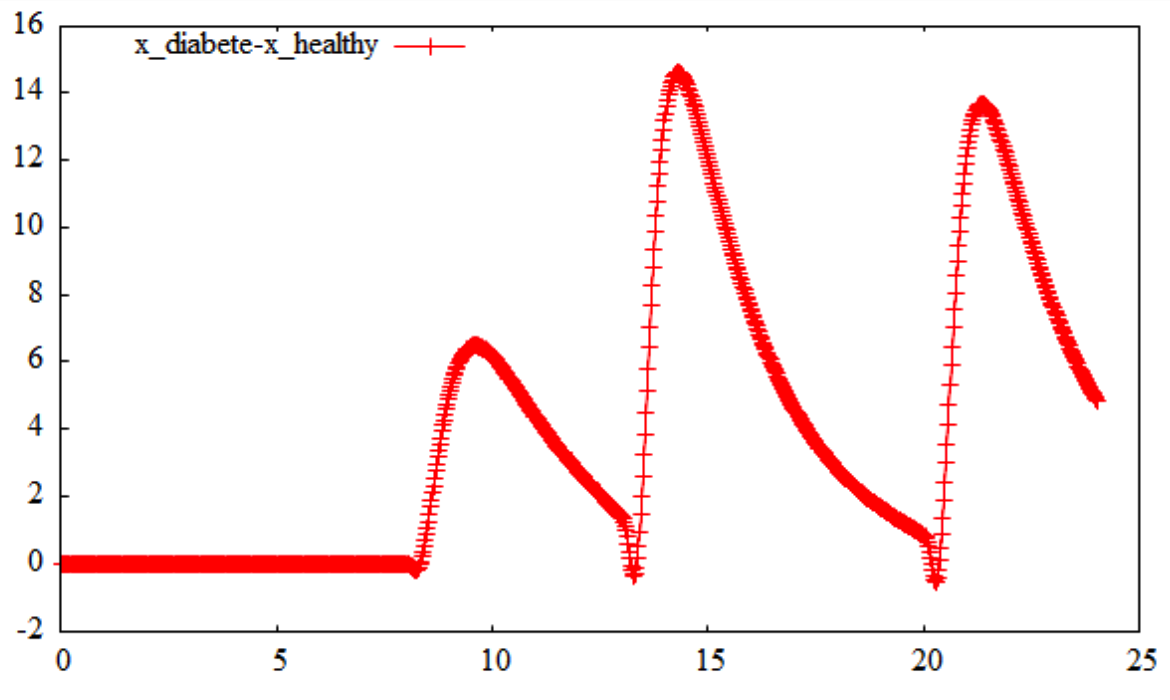
\includegraphics[width=0.7\textwidth]{x_diabete-x_healthy}
\caption{График $x_{diabete}(t)-x_{healthy}(t)$}
\label{task1_dx}
\end{figure}

Репозиторий с решением задания может быть найден по ссылке:
\url{https://github.com/Akhrameev/Practicum_GAMS_1.1}

\newpage


\section{Решение дифференциального уравнения}

\subsection{Постановка задачи}
Система имеет вид:
\begin{equation}\label{syst2_oo}
\ddot{x}(t)=0.2\sqrt{x(t)}-sin(x(t)),\\
x(0)=10; t\in[0,8];
\end{equation}

\subsection{Задача нелинейного программирования}
Переходим к задаче нельнейного программирования, использую разностную схему Эйлера:
\begin{equation}
\frac{x_{k+1}-x_k}{h}=0.2\sqrt{x_k(t)}-sin(x_k(t)), k=1..N\\
x_0=10;
\end{equation}

\subsection{Решение в GAMS}

График $x(t)$ представлен на Рис.~\ref{x_t_task_2_1}

\begin{figure}
\centering
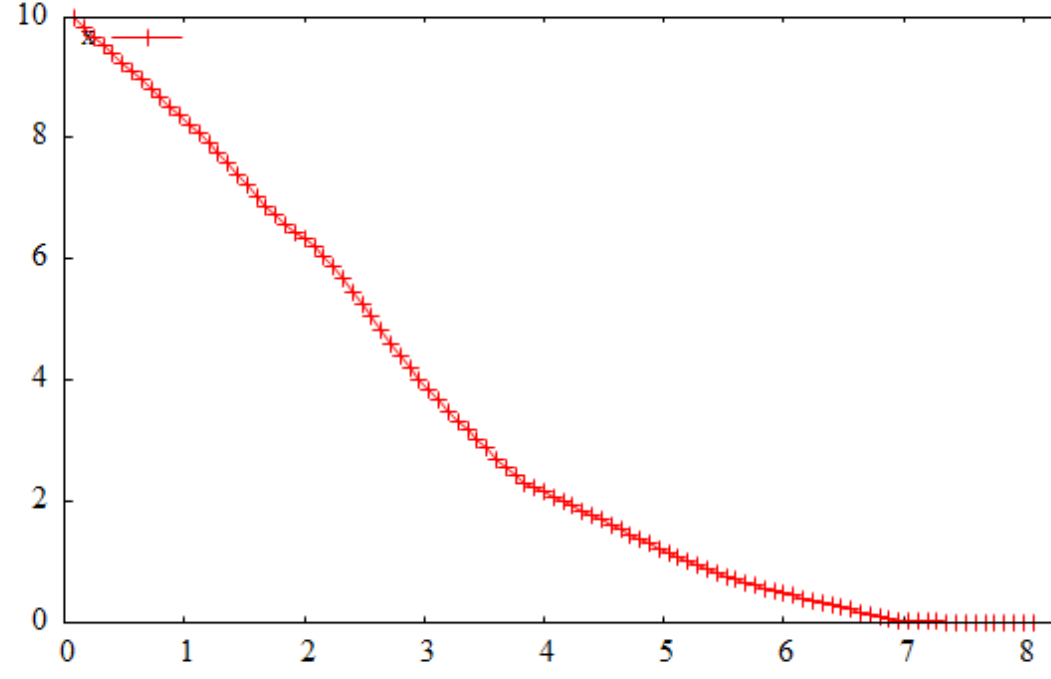
\includegraphics[width=0.7\textwidth]{x_t_task_2_1}
\caption{График $x(t)$}
\label{x_t_task_2_1}
\end{figure}

Репозиторий с решением задания может быть найден по ссылке:
\url{https://github.com/Akhrameev/Practicum_GAMS_2.1}

\section{Задача быстродействия}
\subsection{Постановка задачи}

Система имеет вид:

\begin{equation}\label{syst2}
\left\{ \begin{aligned}
& \ddot{x}+\alpha||\dot{x}||\dot{x} = \rho u, \; x,u \in \textbf{R}^2, \; \alpha,\rho > 0,\;  ||u|| \le 1, \\
& x(0)=x_0, \; \dot{x}(0) = \dot{x}_0, \\
& x(T)=x_T, \; \dot{x}(T) = \dot{x}_T, \\
& T \rightarrow \min_{||u|| \le 1}.
\end{aligned}\right.
\end{equation}

\subsection{Задача нелинейного программирования}

Также, как и в предыдущей задаче, переходим к задаче нелинейного программировани, используя схему Эйлера с шагом $h = \frac{T}{n}$:

\begin{equation}\label{NLP2}
\left\{ \begin{aligned}
& x^1_{k} = x^1_{k-1} + h x^3_{k-1}, \\
& x^2_{k} = x^2_{k-1} + h x^4_{k-1}, \\
& x^3_{k} = x^3_{k-1} + h \Big(-\alpha \sqrt{(x^3_{k-1})^2+(x^4_{k-1})^2} x^3_{k-1} + \rho u^1_{k-1} \Big), \\
& x^4_{k} = x^4_{k-1} + h \Big(-\alpha \sqrt{(x^3_{k-1})^2+(x^4_{k-1})^2} x^4_{k-1} + \rho u^2_{k-1} \Big), \; k = \overline{1,n-1},
\end{aligned}\right.
\end{equation}
с краевыми условиями

$$
    x^1_0 = x^1_0,\; x^2_0 = x^2_0,\; x^3_0 = \dot x^1_0,\; x^4_0 = \dot x^2_0,
$$

$$
    x^1_n = x^1_T,\; x^2_n = x^2_T,\; x^3_n = \dot x^1_T,\; x^4_n = \dot x^2_T.
$$

При этом задача быстродействия ставится при помощи функционала: $h \rightarrow \min$.

\subsection{Решение в GAMS}

Решение задачи при следующих начальных параметрах:

$$
    x^1_0 = -2,\; x^2_0 = 1,\; x^3_0 = 1,\; x^4_0 = 10,
$$

$$
    x^1_n = 0,\; x^2_n = 0,\; x^3_n = 0,\; x^4_n = 0,
$$

$$
    \alpha = 0.1,\; \rho = 1.
$$

Оптимлаьное время $ T = 11.4 $. На Рис. \ref{task2_x}, \ref{task2_u1} и \ref{task2_u2} изображены графики траектории и уравления.

\begin{figure}
\centering
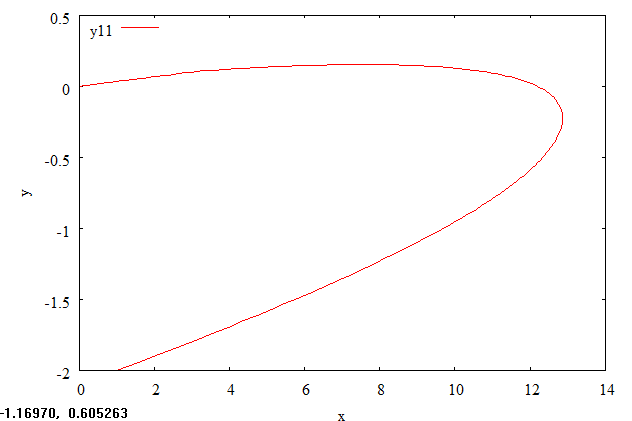
\includegraphics[width=0.7\textwidth]{task2_x}
\caption{График $x(t)$}
\label{task2_x}
\end{figure}

\begin{figure}
\begin{floatrow}
\ffigbox{
    \caption{График $u_1(t)$}
    \label{task2_u1}}
    {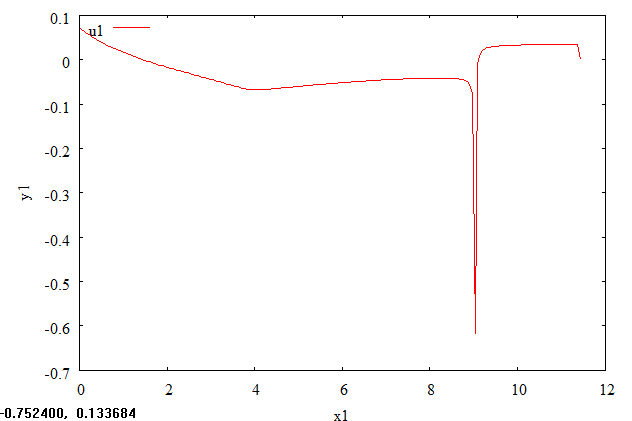
\includegraphics[width=0.5\textwidth]{task2_u1}}
\ffigbox{
    \caption{График $u_2(t)$}
    \label{task2_u2}}
    {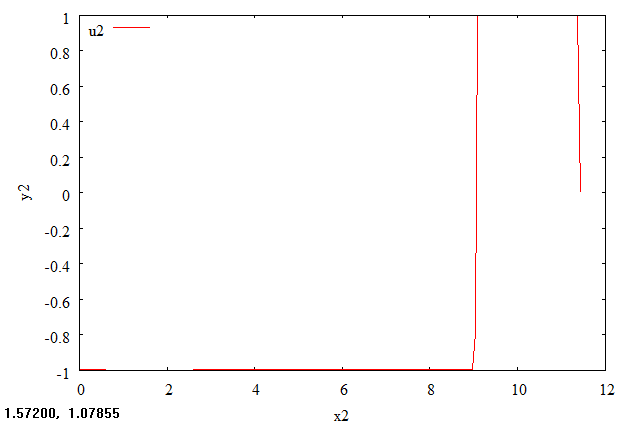
\includegraphics[width=0.5\textwidth]{task2_u2}}
\end{floatrow}
\end{figure}

Репозиторий с решением задания может быть найден по ссылке:
\url{https://github.com/Akhrameev/Practicum_GAMS_3.1}

\newpage

\section{Задача быстродействия с прохождением заданной точки}
\subsection{Постановка задачи}

Система имеет вид:

\begin{equation}\label{syst3}
\left\{ \begin{aligned}
& \ddot{x}+\alpha||\dot{x}||\dot{x} = \rho u, \; x,u \in \textbf{R}^2, \; \alpha,\rho > 0,\;  ||u|| \le 1, \\
& \ddot{y}+\beta||\dot{y}||\dot{y} = \sigma v, \; y,v \in \textbf{R}^2, \; \beta,\sigma > 0,\;  ||v|| \le 1, \\
& x(0)=x^0, \; \dot{x}(0) = \dot{x}^0, \; y(0)=y^0, \; \dot{y}(0) = \dot{y}^0, \\
& x(\tau)=x_t, \tau \in [0,T], \; x(T)=x_T, \\
& T \rightarrow \min_{||u|| \le 1},
\end{aligned}\right.
\end{equation}

Должны выполняться неравенства:

$$
    ||x(t)-y(t)|| \le 2, \; ||x(t)-y(t)|| \ge 1, \; t \in [0,T]. \\
$$


\subsection{Задача нелинейного программирования}

Задача нелинейного программирования записывается при помощи разностной схемы Эйлера с переменным шагом $$h = \begin{cases} \frac{\tau}{n_1}, & k=\overline{1,n_1} \\  \frac{T-\tau}{n_2}, & k=\overline{n_1,n_1+n_2} \end{cases} $$:

\begin{equation}\label{NLP3}
\left\{ \begin{aligned}
& x^1_{k} = x^1_{k-1} + h x^3_{k-1}, \\
& x^2_{k} = x^2_{k-1} + h x^4_{k-1}, \\
& x^3_{k} = x^3_{k-1} + h \Big(-\alpha \sqrt{(x^3_{k-1})^2+(x^4_{k-1})^2} x^3_{k-1} + \rho u^1_{k-1} \Big), \\
& x^4_{k} = x^4_{k-1} + h \Big(-\alpha \sqrt{(x^3_{k-1})^2+(x^4_{k-1})^2} x^4_{k-1} + \rho u^2_{k-1} \Big), \; k = \overline{1,n},
\end{aligned}\right.
\end{equation}

\begin{equation}\label{NLP32}
\left\{ \begin{aligned}
& y^1_{k} = y^1_{k-1} + h y^3_{k-1}, \\
& y^2_{k} = y^2_{k-1} + h y^4_{k-1}, \\
& y^3_{k} = y^3_{k-1} + h \Big(-\beta \sqrt{(y^3_{k-1})^2+(y^4_{k-1})^2} y^3_{k-1} + \sigma v^1_{k-1} \Big), \\
& y^4_{k} = y^4_{k-1} + h \Big(-\beta \sqrt{(y^3_{k-1})^2+(y^4_{k-1})^2} y^4_{k-1} + \sigma v^2_{k-1} \Big), \; k = \overline{1,n}.
\end{aligned}\right.
\end{equation}

Начальные условия остаются такими же, как в предыдущей задаче, с добавлением двух условий: $x_{n_1} = x_t, \; x_{n_1+n_2} = x_T$.

\subsection{Решение в GAMS}

Представлено решение задачи при начальных параметрах:

$$
    x^1_0 = 0,\; x^2_0 = -5,\; x^3_0 = 1,\; x^4_0 = 2, \\
    y^1_0 = 0,\; y^2_0 = -6,\; x^3_0 = 1,\; x^4_0 = 0, \\
$$

$$
    x^1_t = 1,\; x^2_t = -2,\; x^1_T = 0,\; x^2_T = 0.
$$

А также $\rho = \sigma = 4,\; \alpha = \beta = 0.1$.

Оптимлаьное время $ T = 2.1 $. На Рис.\ref{task3_xy}, \ref{task3_u1}, \ref{task3_u2}, \ref{task3_v1} и \ref{task3_v2} изображены графики траекторийи управлений.

\begin{figure}
\centering
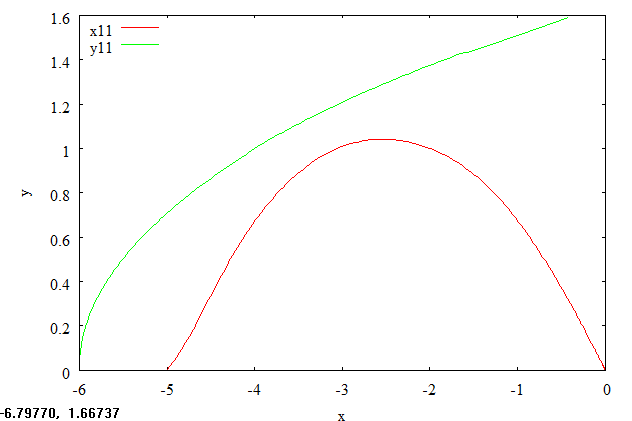
\includegraphics[width=0.7\textwidth]{task3_xy}
\caption{График $x(t)$ è $y(t)$}
\label{task3_xy}
\end{figure}

\begin{figure}
\begin{floatrow}
\ffigbox{
    \caption{График $u_1(t)$}
    \label{task3_u1}}
    {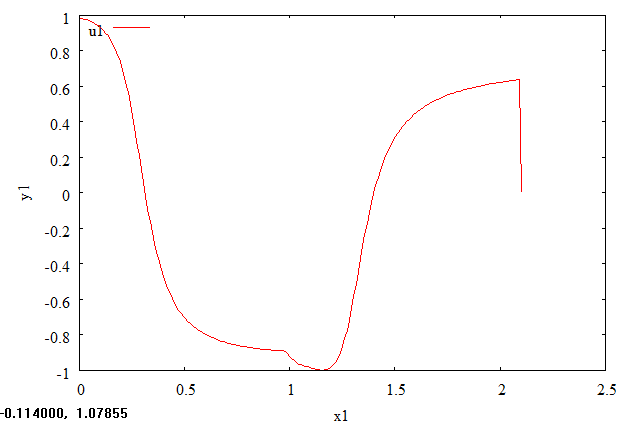
\includegraphics[width=0.5\textwidth]{task3_u1}}
\ffigbox{
    \caption{График $u_2(t)$}
    \label{task3_u2}}
    {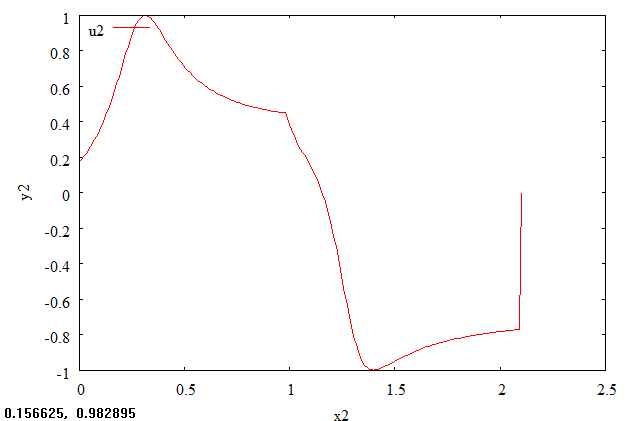
\includegraphics[width=0.5\textwidth]{task3_u2}}
\end{floatrow}
\end{figure}

\begin{figure}
\begin{floatrow}
\ffigbox{
    \caption{График $v_1(t)$}
    \label{task3_v1}}
    {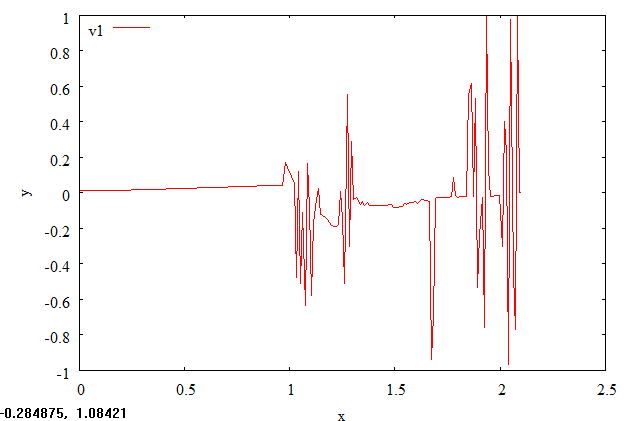
\includegraphics[width=0.5\textwidth]{task3_v1}}
\ffigbox{
    \caption{График $v_2(t)$}
    \label{task3_v2}}
    {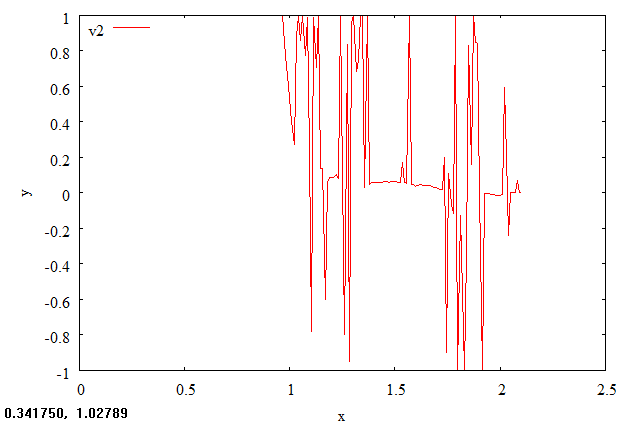
\includegraphics[width=0.5\textwidth]{task3_v2}}
\end{floatrow}
\end{figure}


\newpage
\section{Разработка карьера открытого типа}
\subsection{Постановка задачи}

Динамика разработки карьера описывается следующими уравнениями:

\begin{equation}\label{syst4}
\left\{ \begin{aligned}
& \dot{y} = f^0(u^1,P,Q), \;  y(0)=0, \; y(T) = y_T, \; 0 \le u_1 \le 1, \\
& \dot{P} = u^2, \; P(0) = P^0 \ge 0, \; 0 \le u_2 \le 1,\\
& \dot{Q} = u^2+u^3, \; Q(0) = Q^0 \ge 0, \; 0 \le u_3 \le 1, \\
& J = \int_0^T e^{-\nu t} \Big[ -m f^0 - u^2 - u^3 - p P + s(t)P(2-\frac{P}{f^0}) \Big] dt \rightarrow \max,
\end{aligned}\right.
\end{equation}
где

$$
    f^0(u^1,P,Q) = u^1 P + (1 -u^1) Q.
$$

В задаче $s(t)$ - биржевые цены на сырье взяты из файла $data_r-1.csv$, $p$ - цена переработки единицы сырья, $m$ - цена добычи единицы сырья. Время $T$ не фиксированно.

\subsection{Задача нелинейного программирования}

Перевод задачи \eqref{syst4} в задачу нелинейного программирования:

\begin{equation}\label{NLP4}
\left\{ \begin{aligned}
& y_{k} = y_{k-1} + h f^0_{k-1}, \; y_0 = 0,\; y_n = y_T \\
& P_{k} = P_{k-1} + h u^2_{k-1}, \; P_0 = P^0, \\
& Q_{k} = Q_{k-1} + h (u^2_{k-1} + u^3_{k-1}), \; Q_0 = Q^0, \; k = \overline{1,n}. \\
\end{aligned}\right.
\end{equation}

Функционал:

$$
    J = \sum_{i=0}^n e^{-\nu ih}\Big( -m f^0_i - u^2_i - u^3_i -p P_i + s_i P_i (2-\frac{P_i}{f^0_i}) \Big).
$$


\subsection{Решение в GAMS}

Задача решалась при начальных параметрах:

$$
    m = 1,\;p=5,\;\nu=0.01,\;y_T=2000,\;P^0=0.8,\;Q^0=1.
$$

Получено значение функционала $J = 6.7*10^6$. Графики траектория и управления показаны на Рис.~\ref{task4_P}, \ref{task4_Q}, \ref{task4_y}, \ref{task4_u1}, \ref{task4_u2} и \ref{task4_u3}.

\begin{figure}
\begin{floatrow}
\ffigbox{
    \caption{График $P(t)$}
    \label{task4_P}}
    {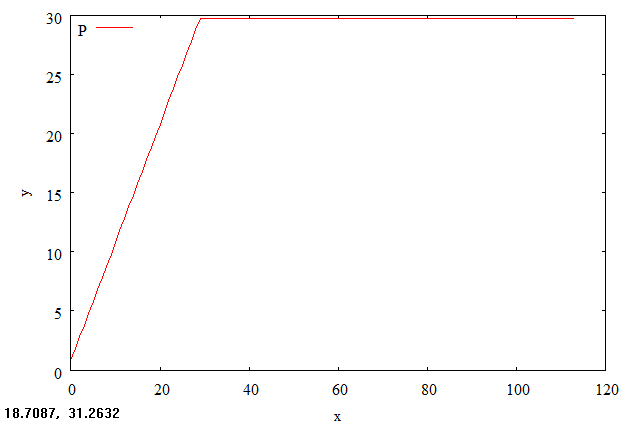
\includegraphics[width=0.5\textwidth]{task4_P}}
\ffigbox{
    \caption{График $Q(t)$}
    \label{task4_Q}}
    {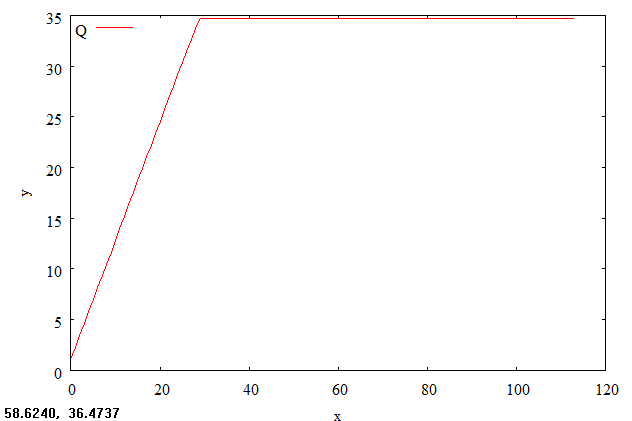
\includegraphics[width=0.5\textwidth]{task4_Q}}
\end{floatrow}
\end{figure}

\begin{figure}
\begin{floatrow}
\ffigbox{
    \caption{График $y(t)$}
    \label{task4_y}}
    {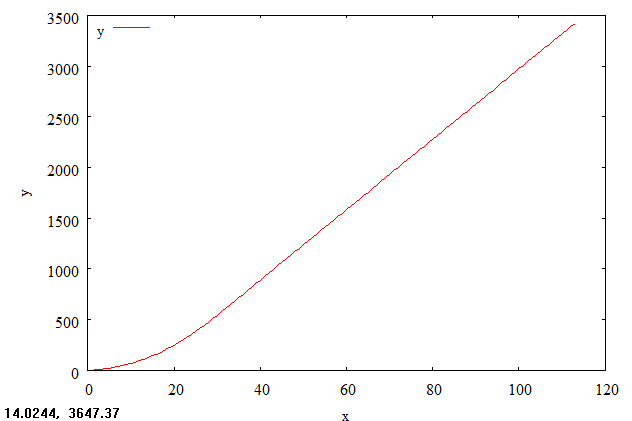
\includegraphics[width=0.5\textwidth]{task4_y}}
\ffigbox{
    \caption{График $u_1(t)$}
    \label{task4_u1}}
    {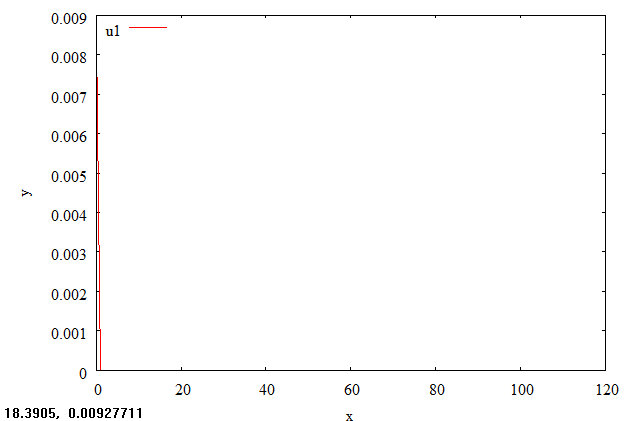
\includegraphics[width=0.5\textwidth]{task4_u1}}
\end{floatrow}
\end{figure}

\begin{figure}
\begin{floatrow}
\ffigbox{
    \caption{График $u_2(t)$}
    \label{task4_u2}}
    {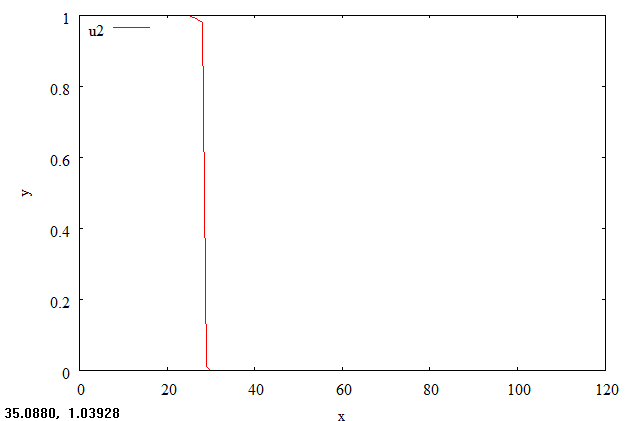
\includegraphics[width=0.5\textwidth]{task4_u2}}
\ffigbox{
    \caption{График $u_3(t)$}
    \label{task4_u3}}
    {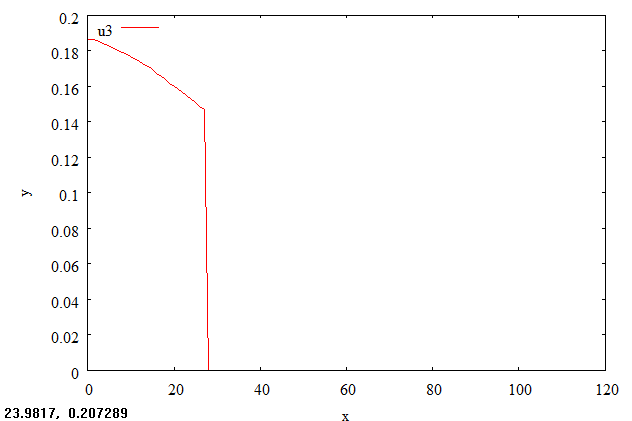
\includegraphics[width=0.5\textwidth]{task4_u3}}
\end{floatrow}
\end{figure}

Репозиторий с решением задания может быть найден по ссылке:
\url{https://github.com/Akhrameev/Practicum_GAMS_5.1}

\newpage

\begin{thebibliography}{0}

\bibitem{Sam} А.А.~Самарский, А.В.~Гулин.
\emph{Численные методы}. Наука, 1989.

\bibitem{Davis} М.Дж.~Дэвис.
\emph{Дифференциальная модель сахарного диабета}.
В книге \emph{Математическое моделирование}. Редакторы Дж.~Эндрюс, Р.~Мак-~Лоун. Мир, 1979.

\bibitem{Cher} Ф.Л.~Черноусько, А.А.~Меликян.
\emph{Игровые задачи управления и поиска}. Наука, 1978.

\bibitem{Aiz} Р.~Айзекс.
\emph{Дифференциальные игры}. Мир, 1967.

\bibitem{Sig} И.Х.~Сигал, А.П.~Иванова.
\emph{Введение в прикладное дискретное программирование}. Физматлит, 2007.


\end{thebibliography}

\end{document}
